\documentclass{beamer}

\mode<presentation> {

% The Beamer class comes with a number of default slide themes
% which change the colors and layouts of slides. Below this is a list
% of all the themes, uncomment each in turn to see what they look like.

%\usetheme{default}
%\usetheme{AnnArbor}
%\usetheme{Antibes}
%\usetheme{Bergen}
%\usetheme{Berkeley}
%\usetheme{Berlin}
%\usetheme{Boadilla}
%\usetheme{CambridgeUS}
%\usetheme{Copenhagen}
%\usetheme{Darmstadt}
%\usetheme{Dresden}
\usetheme{Frankfurt}
%\usetheme{Goettingen}
%\usetheme{Hannover}
%\usetheme{Ilmenau}
%\usetheme{JuanLesPins}
%\usetheme{Luebeck}
%\usetheme{Madrid}
%\usetheme{Malmoe}
%\usetheme{Marburg}
%\usetheme{Montpellier}
%\usetheme{PaloAlto}
%\usetheme{Pittsburgh}
%\usetheme{Rochester}
%\usetheme{Singapore}
%\usetheme{Szeged}
%\usetheme{Warsaw}

% As well as themes, the Beamer class has a number of color themes
% for any slide theme. Uncomment each of these in turn to see how it
% changes the colors of your current slide theme.

%\usecolortheme{albatross}
%\usecolortheme{beaver}
%\usecolortheme{beetle}
\usecolortheme{crane}
%\usecolortheme{dolphin}
%\usecolortheme{dove}
%\usecolortheme{fly}
%\usecolortheme{lily}
%\usecolortheme{orchid}
%\usecolortheme{rose}
%\usecolortheme{seagull}
%\usecolortheme{seahorse}
%\usecolortheme{whale}
%\usecolortheme{wolverine}

%\setbeamertemplate{footline} % To remove the footer line in all slides uncomment this line
%\setbeamertemplate{footline}[page number] % To replace the footer line in all slides with a simple slide count uncomment this line

%\setbeamertemplate{navigation symbols}{} % To remove the navigation symbols from the bottom of all slides uncomment this line
}

\usepackage{extpfeil}
\usepackage{extarrows} %Allows long equation signs
\usepackage{graphicx} % Allows including images
\usepackage{booktabs} % Allows the use of \toprule, \midrule and \bottomrule in tables
\usepackage{physics}
\usepackage{tikz}
\usepackage{cite}
%花体字母
\usepackage{amsthm,amsmath,amssymb}
\usepackage{mathrsfs}
\usepackage{dutchcal}
\usepackage{circuitikz}

%----------------------------------------------------------------------------------------
%	TITLE PAGE
%----------------------------------------------------------------------------------------

\title[University Physics Competition]{Workshop} % The short title appears at the bottom of every slide, the full title is only on the title page

\author{Yanjun Chen} % Your name
\institute[UM-SJTU JI] % Your institution as it will appear on the bottom of every slide, may be shorthand to save space
{
    University of Michigan - Shanghai Jiao Tong University Joint Institute\\% Your institution for the title page
\medskip
}
\date{\today} % Date, can be changed to a custom date

\begin{document}

\begin{frame}
    \titlepage % Print the title page as the first slide
\end{frame}

%----------------------------------------------------------------------------------------
%	 SECTION 1
%----------------------------------------------------------------------------------------

\section{} % Section title slide, unnumbered

\begin{frame}{Read the Whole Problem}
    \vfill
    \begin{itemize}
        \item Decide the problem you want to work on;
        \item Read every question in this problem;
        \item Mark the important points.
    \end{itemize}
    \vfill
\end{frame}


\begin{frame}{Model}
    \begin{itemize}
        \item Research
        \begin{itemize}
            \item Search on Internet;
            \item Use pen and paper to record the details.
        \end{itemize}
        \item Divide your work
        \begin{itemize}
            \item Make sure everyone knows what is your model;
            \item ... % teammate
        \end{itemize}
    \end{itemize}
\end{frame}

\begin{frame}{Coding}
    \begin{itemize}
        \item Choose \textbf{one} easy and powerful programming language;
        \begin{itemize}
            \item MATLAB, Mathematica, R, Python ...
            \item Plotting is the most important step;
            \item There are also some theoretical calculations.
        \end{itemize}
        \item Be familiar with the useful functions (plotting, calculating);
        \item Always save your code and result (git, svn, dropbox ...)!
        \item Organize your work well. The code should be easy to check and modify.
    \end{itemize}
\end{frame}

\begin{frame}{Example}
    \begin{columns}
        \begin{column}{0.5\linewidth}
            \begin{figure}[htbp]
                \centering
                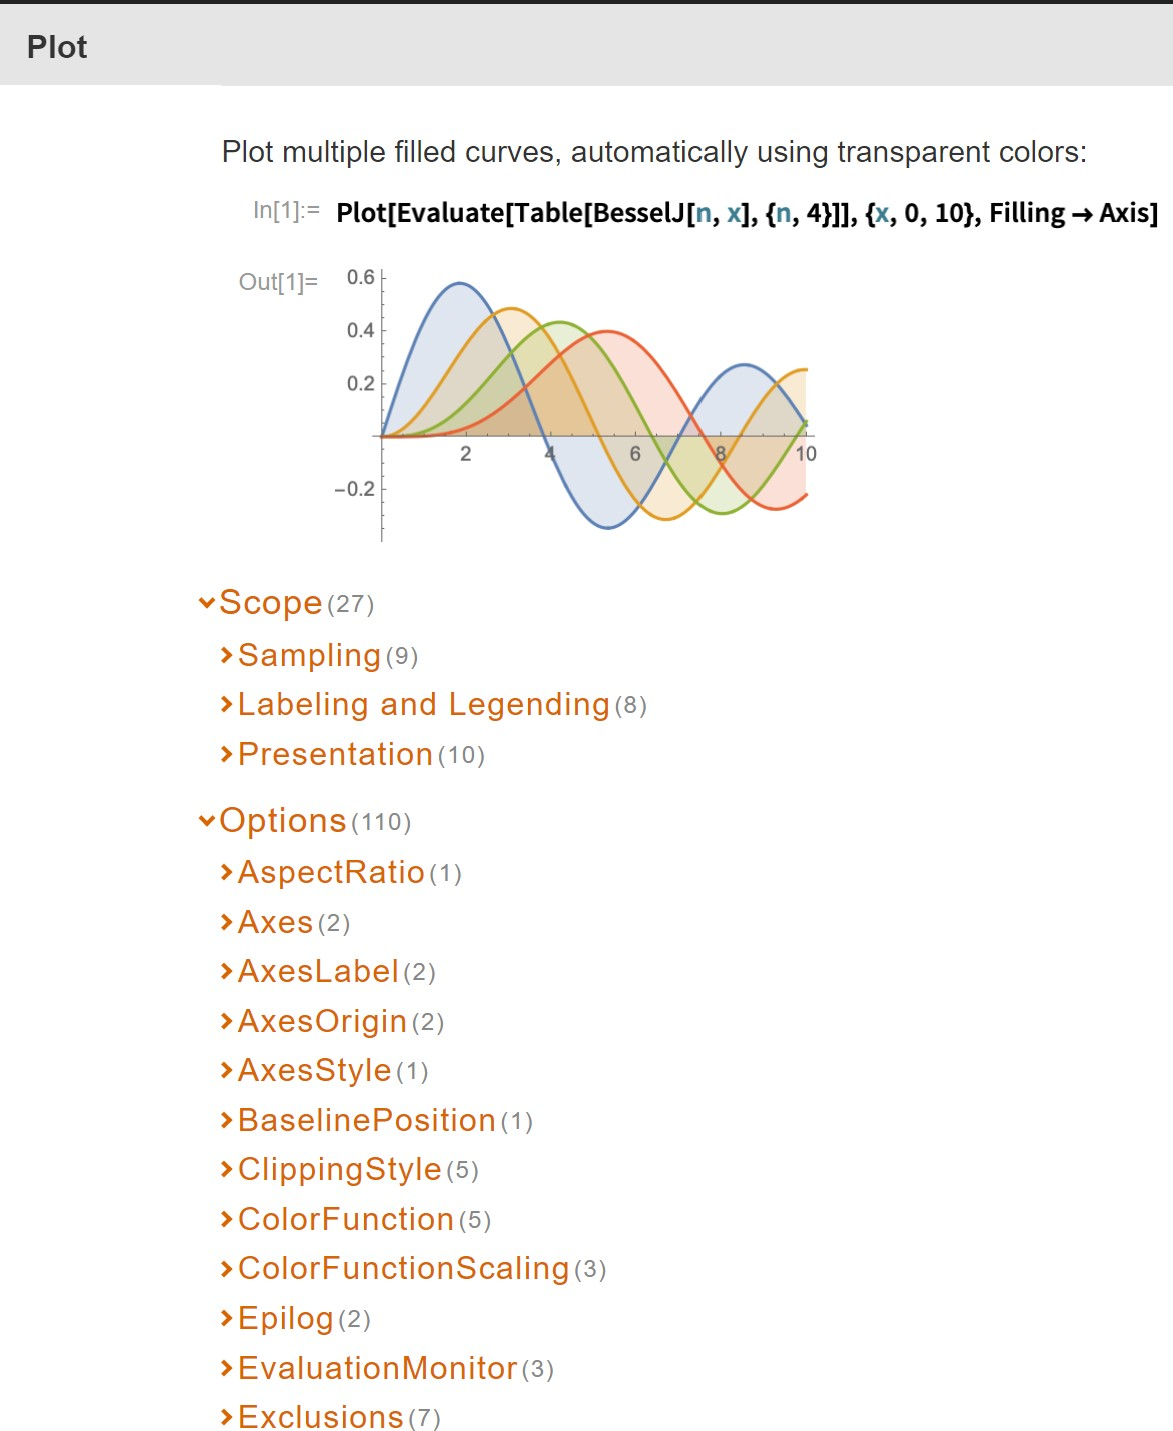
\includegraphics[width=\textwidth]{img/mma_plot.jpg}
            \end{figure}
        \end{column}
        \begin{column}{0.5\linewidth}
            \begin{figure}[htbp]
                \centering
                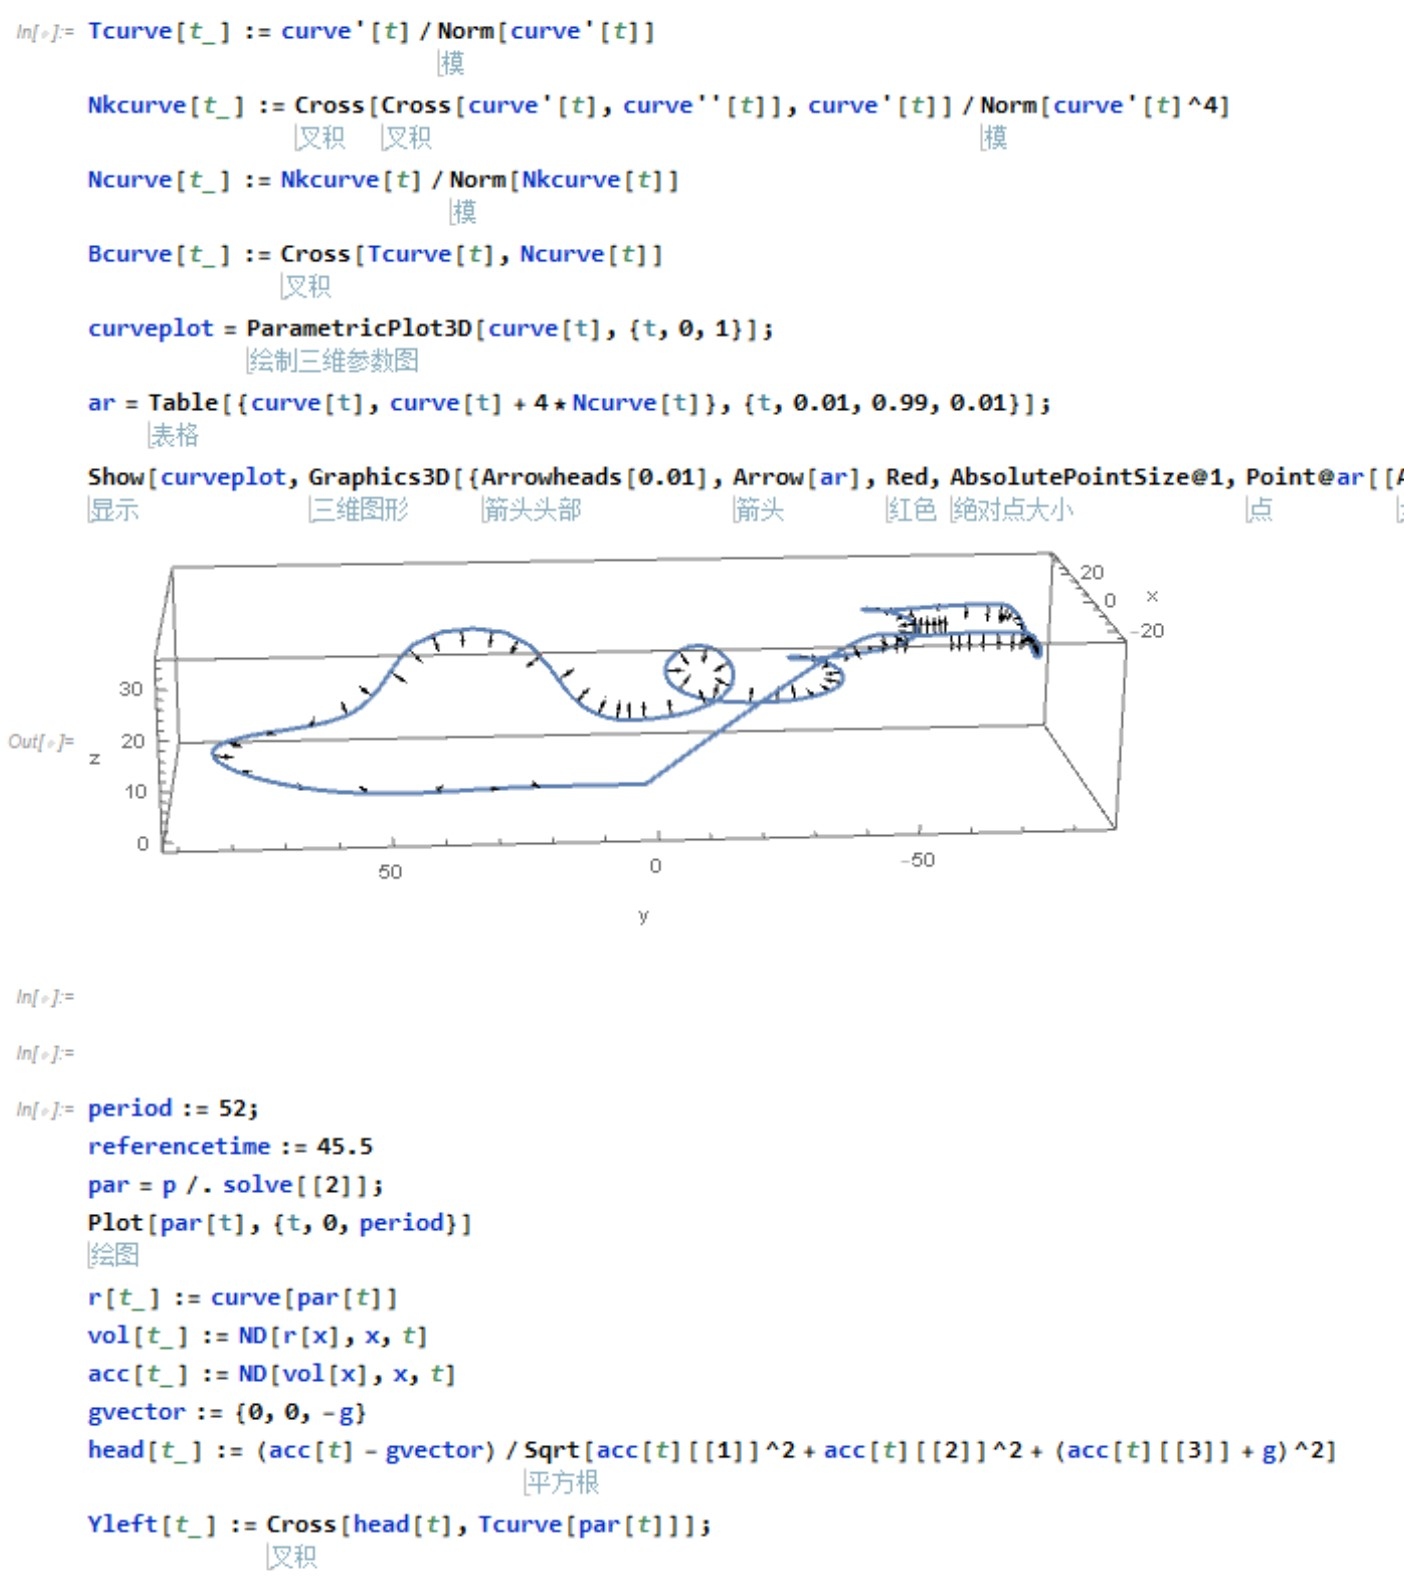
\includegraphics[width=\textwidth]{img/code.jpg}
            \end{figure}
        \end{column}
    \end{columns}
\end{frame}

\begin{frame}{Tools}
    \begin{itemize}
        \item VSCode with extensions;
        \begin{itemize}
            \item LaTeX Workshop (snippets, symbol tables);
            \item Code Spell Checker and Dictionary Completion (check your spelling).
        \end{itemize}
        \item OverLeaf (\url{https://latex.sjtu.edu.cn/});
        \item Markdown Editor (\url{https://notes.sjtu.edu.cn/});
        \item Diagram (\url{https://app.diagrams.net}).      
    \end{itemize}
\end{frame}
%------------------------------------------------





%----------------------------------------------------------------------------------------
%	 CLOSING/SUPPLEMENTARY SLIDES
%----------------------------------------------------------------------------------------

\begin{frame}
    \begin{center}
        \LARGE\bf Have fun in UPC!
    \end{center}
	
\end{frame}


\section{Appendix}

%----------------------------------------------------------------------------------------

\end{document}

